\documentclass[letterpaper ,10pt]{article}

\usepackage[spanish]{babel}
\usepackage[utf8]{inputenc}

\usepackage{fancyhdr}
\usepackage{graphicx}
\graphicspath{ {images/} }
\usepackage{color}
\usepackage{soul}
\usepackage{ulem}
\usepackage{courier}
\usepackage{listings} 

\title{ Proyecto de Planeación enfocado a las Tecnologías de la Información }
\author{Kevin Gordillo Garcia}

\parskip=2mm

\parindent=3mm

\begin{document}


{\centering {\Huge\textbf{ Proyecto de Planeación enfocado a las Tecnologías de la Información} }\par}
{\center {\LARGE{ Fundamentos de la Programación Lógica }} \par}
{\center {\LARGE Catedratica: Doctora Claudia Zepeda Cortes \par} \par}
{\center { \large Alumno: Kevin Gordillo García \par} \par}
{\center {16 de noviembre de 2014 \par} \par}

\newpage

\centerline {\Huge\sffamily\textbf{ Antecedentes  }}

\noindent En la actualidad, los robots comerciales e industriales son ampliamente utilizados, y realizan tareas de forma más exacta o más barata que los humanos. También se les utiliza en trabajos demasiado sucios, peligrosos o tediosos para los humanos. Los robots son muy utilizados en plantas de manufactura, montaje y embalaje, en transporte, en exploraciones en la Tierra y en el espacio, cirugía, armamento, investigación en laboratorios y en la producción en masa de bienes industriales o de consumo. Otras aplicaciones incluyen la limpieza de residuos tóxicos, minería, búsqueda y rescate de personas y localización de minas terrestres.

\vspace{0.5cm}

{\LARGE \textbf{ Robótica educativa}}
\vspace{0.2cm}
\\
La Robótica Educativa es un medio de aprendizaje, en el cual participan las personas que tienen motivación por el diseño y construcción de creaciones propias (objeto que posee características similares a las de la vida humana o animal). Estas creaciones se dan en primera instancia de forma mental y posteriormente en forma física, las cuales son construidas con diferentes tipos de materiales y controladas por un sistema computacional, los que son llamados prototipos o simulaciones. En este contexto, es como vemos se a transformado con el paso del tiempo una competencia de creación de robots prototipo, con un alto enfoque a la parte aplicativa y educativa, la cual se llama: Robocup.\\
\medskip
El RoboCup fue inventado en Japón en 1996 para definir  los grandes retos de la robótica en el futuro, señala, con una competencia nada modesta: un partido de soccer en el 2050 entre jugadores humanos, campeones de la Copa del Mundo, y robots en una situación de igualdad. Con el paso del tiempo, la Robocup se ha convertido en una competencia tecnológica en donde además de la competencia de futbol, se han creado competencias con valor social como actividades de rescate.

\newpage

\centerline {\Huge\sffamily\textbf{ Descripción del problema de Planeación  }}
\vspace{0.5cm}
Se presenta dos extractos de las Reglas de la modalidad de Robot de rescate de Robocup Junior -  Australia de las cuales se basara la narración principal de este problema.\\
\medskip
Reglas de Robot de Rescate – Australia (2014):\\
{\textit {Scenario: A terrible earthquake has hit the city and caused a large chemical storage unit to rupture spilling thousands of litres of toxic chemicals in the centre of the city. There is a person trapped in a sinking rescue capsule (the victim) in the middle of the chemical spill. Rescue crews are having trouble entering the city with the amount of rubble around, and rescue from the air has also been ruled out due to the noxious gases rising from the toxic chemicals directly above the spill. It has been decided that the best form of rescue is the deployment of an autonomous robot that can navigate to the scene, rescue the victim and exit the chemical spill. The robot can be deployed at the start tile (City Limits) or air dropped to any tile that is at least two (2) tile away from the chemical spill (Drop Zone). Primary Rescue: The robot must navigate to the scene and rescue the victim by pushing or dragging the Victim out of the chemical spill. (p. 5) }\\

\medskip
Extracto de síntesis de Robocup Junio Australia:\\
{\textit {Primary Rescue is designed for primary aged students.
Robots compete by following a winding line on a series of tiles to a designated rescue area. On the way the robot could encounter obstacles, bridges and short cut opportunities that will challenge the most intrepid programmer. After negotiating the randomly selected path, the robot arrives at a green coloured area which indicates a chemical spill. While the clock is still ticking the robot must find "the victim" before pushing them out of the quicksand to safety.}

\medskip
{\LARGE \textbf{ Escenario del problema de Planeación}}
\medskip
\\
Basándose en la descripción del escenario, simplificando y delimitando el problema, se concluye el siguiente escenario:\\
\\
Un terrible terremoto ha golpeado a la ciudad de Puebla y ha causado que una gran unidad de almacenaje de químicos se rompiera, esparciendo miles de litros de desechos tóxicos en el centro de la ciudad. Hay una persona atrapada en una capsula de rescate situada en el medio del derrame químico. Los equipos de rescate tienen problemas para entrar a la ciudad con la cantidad de escombros alrededor y rescate por aire también ha sido descartado debido al aumento de gases nocivos producto del derrame tóxico.\\
\\
Se ha decidido que la mejor forma de rescate es el despliegue de un robot autónomo que puede navegar a la escena, rescatar a la víctima y salir del derrame químico. El robot puede desplegarse en los límites de la ciudad o soltarse en el aire a una corta distancia de la zona del derrame químico. 

\vspace{0.5cm}
\medskip
{\LARGE \textbf{ Narración del problema de Planeación}}
\vspace{0.2cm}
\\
Aterrizando en un caso específico se obtiene la siguiente narración:\\
El mini robot es desplegado por aire a una distancia corta del área de desechos tóxicos. El mini robot necesita detectar que se encuentra en la zona del derrame químico vía un sensor de color el cual detectara cuando se entre en la zona del derrame químico caracterizada por ser verde. El robot activa su sistema de localización el cual está basado en un sensor ultrasónico capaz de detectar la distancia a la que están de los objetos enfrente de el a gran distancia. Este sensor está a la altura ideal para detectar la capsula. Además cuenta con un sensor brújula digital con el cual el robot puede detectar la orientación del norte magnético terrestre y así poder ubicar el lugar de la capsula.  Se toma como sistema de referencia la cardinalidad de la zona de despliegue del robot.\\
\\
En este caso el único objeto que está en la zona toxica es la capsula de rescate la cual está situada en el centro de la zona toxica. En este caso no hay obstáculos y el único objetivo del sensor de distancia es detectar la capsula. Cabe destacar que en este caso la zona del derrame y aledañas son totalmente planas, además de estar plenamente delimitada por el color verde. \\ 
\\
Una vez desplegado el robot se le indica a que cardinalidad está situada la capsula tomando como referencia la zona en donde se despliega el robot, en este caso la capsula está situada al sur de la zona de despliegue el robot. El robot procede a activar su sistema, motores y sensores. Después de revisar que no haya ningún problema en su sistema y circuitos el robot, procesada a iniciar el proceso de búsqueda y rescate. \\
\\
Primero el robot detecta que se encuentra en el área no toxica, y que no tiene el objeto, además de identificar su orientación actual, si es diferente de la orientación previamente dada, procede a realizar giros hasta coincidir con la cardinalidad dada. Una vez detectada, procede a moverse hasta llegar al centro del área toxica donde se encuentra la capsula. Una vez estando enfrente de la capsula procede bajar sus pinzas simultáneamente para poder tomar la capsula. Ya que tiene la capsula inicia el proceso de evacuación, en el cual procede a orientarse y moverse al lugar seguro de despliegue, en donde procede a soltar la capsula. Con esto concluye el sistema de búsqueda y rescate del robot.\\
\newpage

\centerline {\Huge\sffamily\textbf{ Desarrollo del Problema de Planeación  }}
\vspace{0.5cm}
\noindent A continuación se presenta el desarrollo de una solución para la narrativa presentada usando programación lógica usando el lenguaje DLV-K. Se presenta el conocimiento previo en el cual se definen el tipo de información y el conocimiento estático.. Consecuentemente se presentan los fluentes del problema, las acciones con sus efectos, las condiciones de efecto representadas en las preposiciones de efecto en sintaxis de lenguaje K. Después se presenta el estado inicial y el estado final del problema. Estos se representan en un autómata. Se finaliza mostrando los planes encontrados.\\
\medskip

{\centerline
{\LARGE \textbf{ Conocimiento Previo (Background Knowledge)}}
}

{\small\texttt{\\
\%Background Knowledge: Este es un modelo sencillo, defino el tipo de informacion y el conocimiento estatico.\\
\%Solo existen tres areas en este problema\\
objeto$(robot)$. objeto$(capsula)$. objeto$(basedespliegue)$.\\
\%Se implementan los cuatro puntos cardinalidades basicos\\
cardinalidad$(sur)$.cardinalidad$(norte)$.cardinalidad$(este)$.cardinalidad$(oeste)$.\\
\%Dos areas en el problema\\
lugar$(centro\_area\_toxica)$. lugar$(area\_segura)$.\\
\%Pinzas que usa el robot para tomar la capsula\\
pinza$(izq)$. pinza$(der)$.\\
 } }

{\centerline
{\LARGE \textbf{ Planificación en K}}
}
\textbf{\noindent \ul{\textsl{Fluentes del problema} }}
\begin{itemize}
\item $orientacion\_objeto(O, C) requires objeto(O), cardinalidad(A):$ Necesario para orientar al robot hacia donde debe moverse.
\item $pocision\_objeto(O, L) requires objeto(O), lugar(L): $ Propiedad que le otorga el conocimiento de saber su pocision dentro del problema.
\item $pinza\_lista(P) requires pinza(P): $Partes del robot que sirven para tomar la capsula.
\item $tener\_capsula:$ Estado necesario para indicar a las pinzas si tienen la capsula.
\item $capsula\_asegurada:$ Estado en donde la capsula a sido asegura y la misión a quedado satisfecho.
\end{itemize}
\vspace{1.8cm}

\textbf{\noindent \ul{\textsl{Acciones del problema} }}
\begin{itemize}
\item $girar\_objeto(O,C) requires objeto(O), cardinalidad(C):$ Acción mediante la cual se cambia la orientacion de los objetos
\item $mover\_hacia(O, L) requires objeto(O), lugar(L):$  Acción mediante la cual se mueve el robot en el problema
\item $desplegar\_pinza(P) requires pinza(P):$Acción mediante la cual se despliegan las pinzas en paralelo haciendo concurrencia con las pinzas
\item $reincorporar\_pinza(P) requires pinza(P):$ Acción mediante la cual se reincorporan las pinzas en paralelo haciendo concurrencia con las pinzas
\item $capturar\_capsula:$Acción en donde se da la orden de capturar la capsula si las pinzas están listas
\item $soltar\_capsula:$ Acción que finaliza la misión de rescate, soltando al capsula en el área segura.
\end{itemize}



\vspace{1.8cm}
\textbf{\noindent \ul{\textsl{ Reglas de Causalidad y condiciones de ejecuci\'on } }}
\begin{itemize}

\item \uuline{Girar después del despliegue del robot}
\\
Para girar el robot, se necesita que la orientación sea la misma que la de la capsula y que no se tenga la capsula. Además que no se puede girar el objeto si previamente se está girando en otra dirección y no se puede girar mientras se mueve el robot. Lo que causa que el robot cambie de orientación.

\item \uuline{Mover después de girar}
\\
Para mover el robot, se necesita que posición a la que se moverá sea diferente a  la actual. Además que no se pude mover el robot si no tiene la misma dirección que la capsula y si el robot se está moviendo no puede girar a la vez. Lo que causa que el robot cambie de posición.

\item \uuline{Despliegue de pinzas}
\\
Las pinzas del robot se despliegan en paralelo cuando se detecta que el robot y el la casual están en el mismo lugar. Con esto habilitaremos las pinzas para poder capturar la capsula. No se puede realizar ningún otro proceso mientras se despliegan las pinzas

\item \uuline{Captura de la capsula}
\\
La captura del objeto se realiza cuando las pinzas están desplegadas y listas para usarse. Esto causa que se capture la capsula. No se puede realizar ningún otro proceso mientras se captura la capsula

\item \uuline{Girar después de la captura}
\\
Después de la captura el robot necesita regresar a la zona de despliegue. Para esto primero tiene que girar hacia la orientación de la base de despliegue. Al mismo tiempo que se mueve el robot va moviendo la capsula que tiene capturada. Cumple las mistas condiciones de no ejecución que el girar después del despliegue con la capsula.

\item \uuline{Mover después de girar con la capsula}
\\
El robot una vez orientado a la orientación de la base de despliegue procede a moverse. Esto causa que el robot cambie de posición junto con al capsula.

\item \uuline{Soltar Capsula y reincorporación de pinzas}
\\
Finalmente el robot procede a soltar la capsula en el área segura, para después reincorporar sus pinzas para así volver al estado en que se desplego y poder realizar la recuperación del robot con éxito

\bigskip
\item La base de despliegue no puede cambiar de orientación ni de posición en el proceso del problema bajo ninguna circunstancia.
\item Por inercia, el robot asume que las propiedades de orientación, posición, pinzas, tener capsula y casual asegurada; permanecerán sin cambio por default.
\end{itemize}


\textbf{\noindent \ul{\textsl{Estado inicial} }}
\\
\\
El estado inicial del problema es el siguiente: El robot se encuentra en el área segura con una orientación al norte (la base de despliegue se encuentra con las mismas propiedades), el cual no tiene la capsula en sus pinzas. La capsula se encuentra en el área toxica orientada al sur. La capsula no está segura.
\vspace{0.5cm}
\\
\textbf{\noindent \ul{\textsl{Estado final} }}
\\
\\
El objetivo es tener la capsula asegurada y regresar al robot a su estado de despliegue, es decir con las pinzas reincorporadas en. El plan no debe de durar más de 8 pasos.
\\

\newpage


\centerline {\Huge\sffamily\textbf{Autómata (Grafo de transición de estados)  }}
\vspace{0.5cm}
\noindent Debido a que el total de fluentes para este problema es de 16 positivos y 32 estados contando la negación de cada estado positivo, la cantidad de estados que se tendría en el problema sería de 232 en el cual nos da: 4294967296 estados posibles. La cantidad que sería necesario representar es muy grande, por lo cual, solo se presentara el autómata que representa el estado final del problema.

\begin{figure*}[htb]
\hspace*{-4cm} 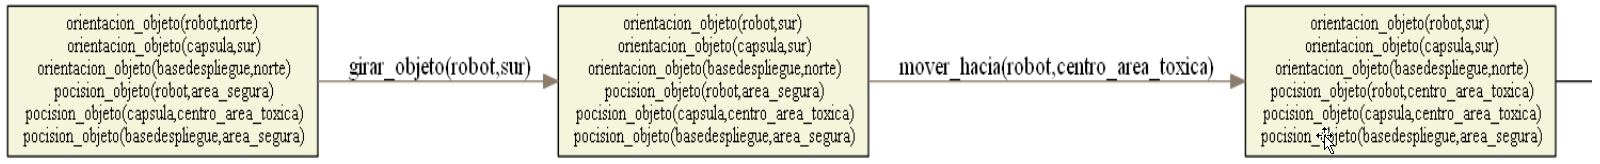
\includegraphics[width=1.7\textwidth]{g1}
\caption{Automata Primera parte de cuatro }
\end{figure*}

\begin{figure*}[htb]
\hspace*{-4.5cm} 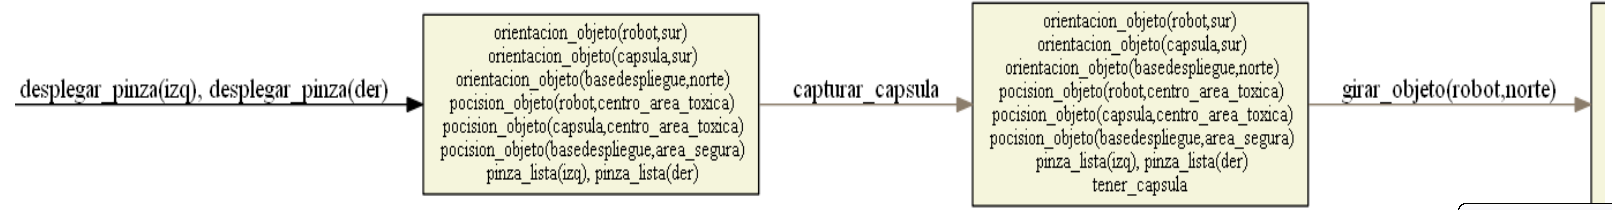
\includegraphics[width=1.7\textwidth]{g2}
\caption{Automata Segunda parte de cuatro }
\end{figure*}

\begin{figure*}[htb]
\hspace*{-4.5cm} 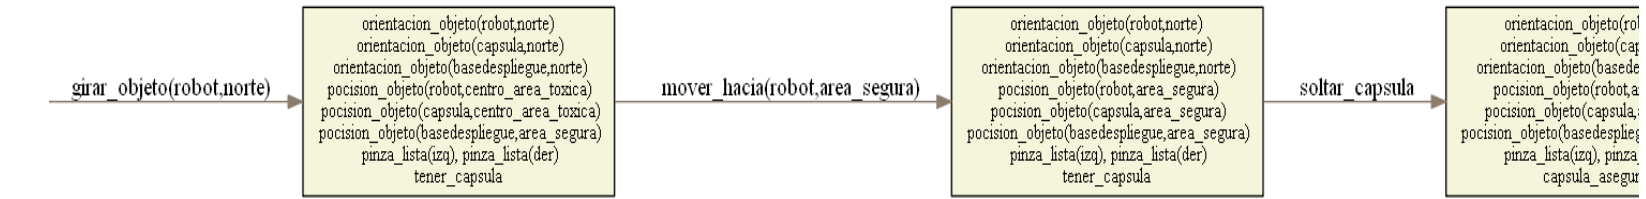
\includegraphics[width=1.7\textwidth]{g3}
\caption{Automata Segunda parte de cuatro }
\end{figure*}

\begin{figure*}[htb]
\hspace*{-3cm} 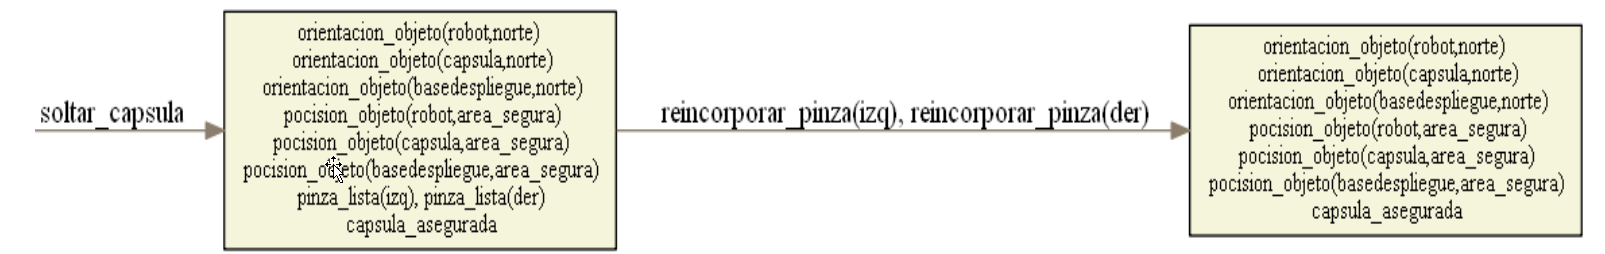
\includegraphics[width=1.5\textwidth]{g4}
\caption{Automata Segunda parte de cuatro }
\end{figure*}

\newpage
Debido a la dimension del grafo, se tuvo que recortar en 4 partes. El codigo del grafo asi como su imagen de salida PNG, estan adjuntos a este trabajo.
\vspace{2cm}
\\


\newpage
\centerline {\Huge\sffamily\textbf{Programación Lógica: Planificación en K }}
\vspace{0.5cm}
\noindent A continuación se muestran los códigos desarrolladores en el lenguaje de programación lógica DLV-K. Se adjuntan dos archivos, el conocimiento previo así como el archivo principal de planning.

\vspace{1cm}
{\centerline 
{ \large \textbf{ Planning\_RobotRescue\_KevinGordillo.bk (Background Knowledge)}
}

\noindent \small \texttt{\%Background Knowledge: Este es un modelo sencillo, defino el tipo de informacion y el conocimiento estatico.\\ 
\%Solo existen tres areas en este problema\\
objeto$(robot)$. objeto$(capsula)$. objeto$(basedespliegue)$.\\
\%Se implementan los cuatro puntos cardinalidades basicos\\
cardinalidad$(sur)$.cardinalidad$(norte)$.cardinalidad$(este)$.cardinalidad$(oeste)$.\\
\%Dos areas en el problema\\
lugar$(centro\_area\_toxica)$. lugar$(area\_segura)$.\\
\%Pinzas que usa el robot para tomar la capsula\\
pinza$(izq)$. pinza$(der)$.\\
 } 

\vspace{1cm}
{\centerline 
{ \large \textbf{Planning\_RobotRescue\_KevinGordillo.plan $(Main Planning)$}
}

{\noindent \tiny {
\begin{lstlisting}%Planning of Robot Rescue-By Kevin Gordillo
%Planeacion de Robot Rescate -Por Kevin Gordillo


fluents:
	orientacion_objeto(O, C) requires objeto(O), cardinalidad(A).
	%Necesario para orientar al robot hacia donde debe moverse
	pocision_objeto(O, L) requires objeto(O), lugar(L). 			
%Propiedad que le otorga el conocimiento de saber su pocision dentro del problema
	pinza_lista(P) requires pinza(P).								
%Partes del robot que sirven para tomar la capsula
	tener_capsula.													
%Estado necesario para indicar a las pinzas si tienen la capsula
	capsula_asegurada.												
%Estado en donde la capsula a sido asegura y la mision a quedado satisfecha	
	
actions:
	girar_objeto(O,C) requires objeto(O), cardinalidad(C).			
%Accion mediante la cual se cambia la orientacion de los objetos
	mover_hacia(O, L) requires objeto(O), lugar(L).					
%Accion mediante la cual se mueve el robot en el problema
	desplegar_pinza(P) requires pinza(P).							
%Accion mediante la cual se despliegan las pinzas en paralelo haciendo concurrencia con las pinzas
	reincorporar_pinza(P) requires pinza(P).						
%Accion mediante la cual se reincorporan las pinzas en paralelo haciendo concurrencia con las pinzas
	capturar_capsula.											
	%Accion en donde se da la orden de capturar la capsula si las pinzas estan listas
	soltar_capsula.													
%Accion que finaliza la mision de rescate, soltando al capsula en el area segura.

	%Reglas de Causalidad y condiciones de ejecucion
always:
	%GIRAR - SIN CAPSULA
	caused orientacion_objeto(robot, L) after girar_objeto(robot,L),
 not tener_capsula. %la orientacion cambia si giramos el robot
	caused -orientacion_objeto(robot, L) after girar_objeto(robot,L1), orientacion_objeto(robot, L),
 not tener_capsula.
	executable girar_objeto(robot, L1)	if orientacion_objeto(robot,L), orientacion_objeto(capsula, L1),
L<>L1, not tener_capsula. 
%solo se ejectua el girar si las orientaciones son diferentes
	nonexecutable girar_objeto(robot,P) if girar_objeto(robot,P1), P<>P1, not tener_capsula.
	nonexecutable girar_objeto(robot,P) if mover_hacia(robot,L), not tener_capsula.  %No puedes girar y
 moverte al mismo tiempo
	
	%MOVER ROBOT -- SIN CAPSULA	
	caused pocision_objeto(robot, L) after mover_hacia(robot, L),not tener_capsula. %la pocision cambia
 si se mueve el robot
	caused -pocision_objeto(robot, L) after  mover_hacia(robot, L1), pocision_objeto(robot, L), L<>L1,
not tener_capsula.
	executable mover_hacia(robot,P) if not pocision_objeto(robot, P), not tener_capsula. 
	nonexecutable mover_hacia(robot,P) if orientacion_objeto(robot,L), orientacion_objeto(capsula, L1),
 L<>L1.
	nonexecutable mover_hacia(robot,P) if girar_objeto(robot, L). %No puedes  avanzar y girar

	
	%DESPLEGARSE PINZAS -- PARALELAMENTE
	%se despliegan las pinzas si no se tiene la capsula, las pinzas no estan listas y la capsula y el robot 
estan en el mismo lugar
	executable desplegar_pinza(P) if pocision_objeto(robot, L), pocision_objeto(capsula,L),
 not tener_capsula, not pinza_lista(I), not pinza_lista(D). 
	nonexecutable desplegar_pinza(P) if girar_objeto(robot, C).
	nonexecutable desplegar_pinza(P) if mover_hacia(robot,L).
	nonexecutable desplegar_pinza(P) if pinza_lista(izq), pinza_lista(der).
	nonexecutable desplegar_pinza(P) if capturar_capsula.
	nonexecutable desplegar_pinza(P) if tener_capsula.
	caused pinza_lista(P) after desplegar_pinza(P).
	
	%CAPTURAR OBJETO
	caused tener_capsula after capturar_capsula.
	executable capturar_capsula if pinza_lista(I), pinza_lista(D), I<>D. %Si las pinzas estan listas se procede 
a capturar la capsula
	nonexecutable capturar_capsula if mover_hacia(O,L).
	nonexecutable capturar_capsula if girar_objeto(O,C).
	nonexecutable capturar_capsula if desplegar_pinza(P).
	nonexecutable capturar_capsula if not pinza_lista(I), not pinza_lista(D).
	
	%GIRAR A ZONA DE DESPLEGARSE -- CON CAPSULA
	caused orientacion_objeto(robot, L) after girar_objeto(robot, L), tener_capsula.
	caused -orientacion_objeto(robot, L) after girar_objeto(robot, L1),  orientacion_objeto(robot, L),
 tener_capsula.
	caused orientacion_objeto(capsula, L) after girar_objeto(robot, L), tener_capsula.
	caused -orientacion_objeto(capsula, L) after girar_objeto(robot, L1),  orientacion_objeto(capsula, L),
 tener_capsula.
	executable girar_objeto(robot, L1)	if orientacion_objeto(robot,L),
 orientacion_objeto(basedespliegue, L1), 
L<>L1,
 tener_capsula.%Se toma como referencia la zona de despliegue para regresar
	nonexecutable girar_objeto(robot,P) if girar_objeto(robot,P1), P<>P1.
	nonexecutable girar_objeto(robot,P) if mover_hacia(robot,L). %NO GIRAR NI MOVER AL MISMO TIEMPO
	
	
	%MOVERSE A ZONA DE DESPLEGARSE -- CON CAPSULA
	caused pocision_objeto(robot, L) after mover_hacia(robot, L), tener_capsula.
	caused -pocision_objeto(robot, L) after  mover_hacia(robot, L1), pocision_objeto(robot, L), L<>L1,
 tener_capsula.
	caused pocision_objeto(capsula, L) after mover_hacia(robot, L), tener_capsula.
	caused -pocision_objeto(capsula, L) after tener_capsula, mover_hacia(robot, L1), 
 pocision_objeto(capsula, L), L<>L1.
	executable mover_hacia(robot,P) if not pocision_objeto(robot, P),  tener_capsula. 
	nonexecutable mover_hacia(robot,P) if orientacion_objeto(robot,L),
 orientacion_objeto(basedespliegue, L1),
 L<>L1, 
tener_capsula. %Se toma como referencia la zona de despliegue para regresar

	%SOLTAR CAPSULA
	caused -tener_capsula after soltar_capsula.
	caused capsula_asegurada after soltar_capsula.
	executable soltar_capsula if pocision_objeto(capsula, area_segura), tener_capsula.
	nonexecutable soltar_capsula if mover_hacia(robot, L).
	nonexecutable soltar_capsula if girar_objeto(robot, L).
	nonexecutable soltar_capsula if capturar_capsula.
	
	%REINCORPORAR PINZAS -- PARALELAMENTE
	caused -pinza_lista(P) after reincorporar_pinza(P).
	executable reincorporar_pinza(P) if capsula_asegurada, pocision_objeto(robot, area_segura), 
not tener_capsula, pinza_lista(I), pinza_lista(D), I<>D.
	nonexecutable reincorporar_pinza(P) if girar_objeto(robot, C).
	nonexecutable reincorporar_pinza(P) if mover_hacia(robot,L).
	nonexecutable reincorporar_pinza(P) if  not pinza_lista(izq), not pinza_lista(der).
	nonexecutable reincorporar_pinza(P) if  capturar_capsula.
	
	%PROHIBIMOS DE POCISION DE BASE DESPLIEGUE 
	%Impedimos que las propiedades de la base de despligue cambien en el proceso del problema.
	forbidden not pocision_objeto(basedespliegue,area_segura). 
	forbidden not orientacion_objeto(basedespliegue,norte).

	%INERCIAS: Asumimos que los sigueintes fluentes permancen sin cambio por default.
	inertial orientacion_objeto(O,L). 	
	inertial pocision_objeto(O,L).  
	inertial pinza_lista(P).
	inertial tener_capsula.
	inertial capsula_asegurada.
	
	%Restricciones del estado inicial
initially:
	-capsula_asegurada.
	-tener_capsula.
	pocision_objeto(capsula,centro_area_toxica).
	orientacion_objeto(capsula, sur).
	pocision_objeto(robot,area_segura).
	orientacion_objeto(robot, norte).
	pocision_objeto(basedespliegue,area_segura).
	orientacion_objeto(basedespliegue, norte).
	
	%El objetivo estara resuleto cuando la capsula este asegurada y el robot vuelva a su 
estado inicial en 8 estados
goal: capsula_asegurada, -pinza_lista(izq),-pinza_lista(der) ? (8) 


\end{lstlisting}
}}

\newpage

{\centerline 
{ \large \textbf{ Resultados de la compilación del programa }
}

\noindent Para usar el programa se define el uso del programa DLV, seguido del archivo background junto con
 su archivo de planning, especificando que es un programa de planning fron-end, y por ultimo definiendo el número máximo de enteros de usar el programa.

\small{
\begin{lstlisting}
C:\Users\alex\Copy\ITI\6to_Cuatri\ProgramacionLogica\ProyectoRobotrescue>
dlv Planning_RobotRescue_KevinGordillo.bk Planning _RobotRescue_KevinGordillo.plan
 -FP -N=8


STATE 0: -capsula_asegurada,orientacion_objeto(robot,norte),
orientacion_objeto(capsula,sur),orientacion_objeto(basedespliegue,norte),
 pocision_objeto(robot,area_segura), pocision_objeto(capsula,centro_area_toxica),
 pocision_objeto(basedespliegue,area_segura), -tener_capsula

ACTIONS: girar_objeto(robot,sur)

STATE 1: pocision_objeto(robot,area_segura), 
pocision_objeto(capsula,centro_area_toxica), 
pocision_objeto(basedespliegue,area_segura), 
-orientacion_objeto(robot,norte), orientacion_objeto(capsula,sur), 
orientacion_objeto(basedespliegue,norte),
 orientacion_objeto(robot,sur)

ACTIONS: mover_hacia(robot,centro_area_toxica)

STATE 2: pocision_objeto(robot,centro_area_toxica), 
-pocision_objeto(robot,area_segura),
 pocision_objeto(basedespliegue,area_segura), 
pocision_objeto(capsula,centro_area_toxica), orientacion_objeto(capsula,sur),
orientacion_objeto(basedespliegue,norte), orientacion_objeto(robot,sur)

ACTIONS: desplegar_pinza(izq), desplegar_pinza(der)

STATE 3: pocision_objeto(robot,centro_area_toxica), 
pocision_objeto(capsula,centro_area_toxica), 
pocision_objeto(basedespliegue,area_segura),
 pinza_lista(izq), pinza_lista(der),
 orientacion_objeto(capsula,sur), 
orientacion_objeto(basedespliegue,norte), orientacion_objeto(robot,sur)

ACTIONS: capturar_capsula

STATE 4: pocision_objeto(robot,centro_area_toxica), tener_capsula,
 pocision_objeto(capsula,centro_area_toxica),
 pocision_objeto(basedespliegue,area_segura), 
pinza_lista(izq), pinza_lista(der), orientacion_objeto(capsula,sur), 
orientacion_objeto(basedespliegue,norte), orientacion_objeto(robot,sur)

ACTIONS: girar_objeto(robot,norte)

STATE 5: pocision_objeto(robot,centro_area_toxica),
 tener_capsula, pocision_objeto(capsula,centro_area_toxica),
pocision_objeto(basedespliegue,area_segura),
pinza_lista(izq), pinza_lista(der), orientacion_objeto(robot,norte),
-orientacion_objeto(capsula,sur), orientacion_objeto(basedespliegue,norte),
 -orientacion_objeto(robot,sur), orientacion_objeto(capsula,norte)

ACTIONS: mover_hacia(robot,area_segura)

STATE 6: tener_capsula, pocision_objeto(robot,area_segura), 
-pocision_objeto(robot,centro_area_toxica), 
-pocision_objeto(capsula,centro_area_toxica),
 pocision_objeto(basedespliegue,area_segura), 
pinza_lista(izq), pinza_lista(der), pocision_objeto(capsula,area_segura),
 orientacion_objeto(robot,norte), orientacion_objeto(basedespliegue,norte), 
orientacion_objeto(capsula,norte)

ACTIONS: soltar_capsula

STATE 7: pocision_objeto(robot,area_segura), 
pocision_objeto(basedespliegue,area_segura), 
pinza_lista(izq), pinza_lista(der), pocision_objeto(capsula,area_segura), 
-tener_capsula,capsula_asegurada, orientacion_objeto(robot,norte),
orientacion_objeto(basedespliegue,norte), orientacion_objeto(capsula,norte)

ACTIONS: reincorporar_pinza(izq), reincorporar_pinza(der)

STATE 8: pocision_objeto(robot,area_segura),
pocision_objeto(basedespliegue,area_segura), -pinza_lista(izq),
-pinza_lista(der), pocision_objeto(capsula,area_segura), 
capsula_asegurada, orientacion_objeto(robot,norte), 
orientacion_objeto(basedespliegue,norte), orientacion_objeto(capsula,norte)

PLAN: girar_objeto(robot,sur); mover_hacia(robot,centro_area_toxica);
 desplegar_pinza(izq), desplegar_pinza(der); captur
ar_capsula; girar_objeto(robot,norte); mover_hacia(robot,area_segura);
 soltar_capsula; reincorporar_pinza(izq), reincorp
orar_pinza(der)

Check whether that plan is secure (y/n)? y
The plan is secure.
\end{lstlisting}

}
\begin{figure*}[htb]
\hspace*{-3cm} 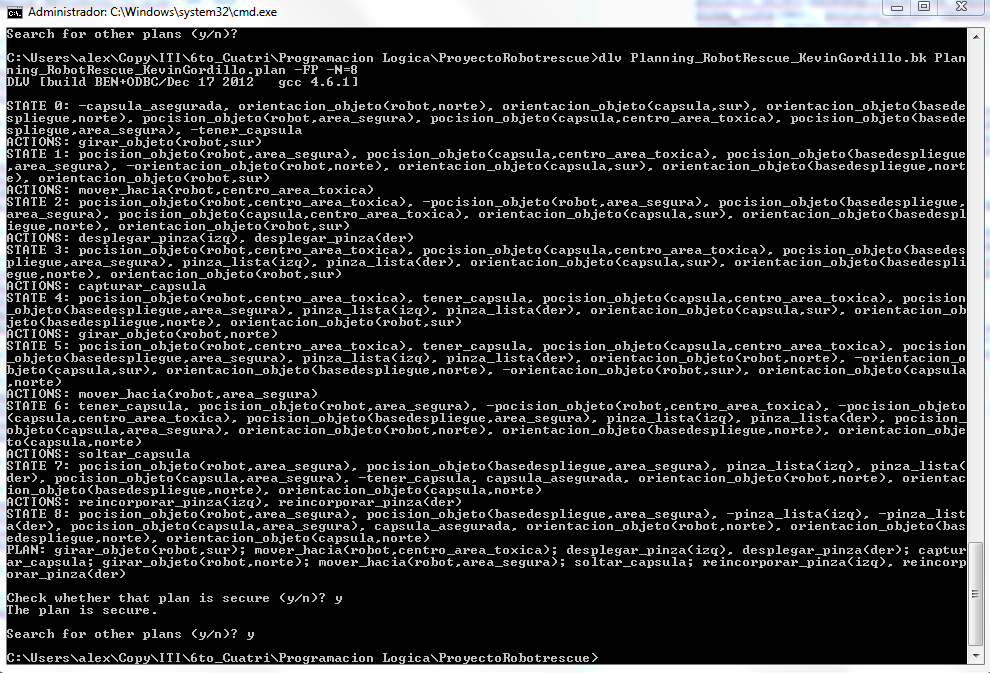
\includegraphics[width=1.5\textwidth]{compile}
\caption{Compilacion}
\end{figure*}

\newpage
.
\\
\newpage

\centerline {\Huge\sffamily\textbf{Conclusión  }}
\vspace{0.5cm}
\noindent Se aplicaron y se reforzaron los conocimientos acerca de planning implementándolo en un ejemplo del área de las TI’s. En el cual empezando desde una situación o estado inicial, se deseó llegar a un objetivo, teniendo a nuestra disposición una serie de acciones. De esta manera se encontró una apropiada secuencia de acciones, llamado plan que cuando es ejecutado lleva al objetivo.

La implementación previamente indicia fue hecha en un área muy estudiada de las tecnologías de la Información: la Robótica, en este caso aterrizando en un área técnicamente limitada que es la robótica educativa para niños. En este ejemplo se presentó el problema que se otorga en las competencias internacionales de creación de robots autóctonos en la categoría Junior. Se trata de acondicionar y programar un robot para que pueda rescatar después de un desastre químico, una capsula donde se encuentran personas, y ponerla en un lugar seguro. Para este proyecto se tuvo que delimitar a gran medida la narración base de este problema para poderlo implementar.

Con esto se consiguió resolver el problema planteado mediante el diseño y modelado de la programación lógica declarativa, donde el programador solo define las los fluentes y las reglas a seguir en el programa. Este tipo de programación y en especial DLVK nos permite representar el conocimiento incompleto y llegar a una solución a partir de algunos hechos verdaderos.

En los resultados se puede notar como se lograr establecer un plan eficiente para la realización de esta tarea por el robot, planteando las bases para poder seguir escalando el problema y resolver problemas más complejos.

\newpage
\centerline {\Huge\sffamily\textbf{Bibliografía }}
\begin{lstlisting}

Robot Rescue.
Polleres, A. (2004). Planning under Uncertainty with Action Languages:
 A Logic Programming Approach. University of Calabria
CeroN, O. Ejemplos DLVK. 
Gerald (2004) DLVK.
Faber, W. (2001). Logic Programming and Nonmonotonic Reasoning
Vlahavas, I. (2004). Intelligent Techniques for Planning



\end{lstlisting}



\end{document}